% =============================================================================
% BRENT Pattern System v3 — Detector de canales de tendencia sobre el Brent
% Documentación de proyecto (formato académico). Compilar en Overleaf:
%   pdflatex main + bibtex main + pdflatex ×2  (o latexmk -pdf main.tex)
% Requiere la carpeta figures/ adjunta (todas las figuras se generan a partir
% de los resultados reales de results/reports y results/predictions).
% =============================================================================
\documentclass[11pt,a4paper]{article}
\usepackage[utf8]{inputenc}
\usepackage[T1]{fontenc}
\usepackage[spanish,es-nodecimaldot]{babel}
\usepackage{lmodern}
\usepackage{microtype}
\usepackage{geometry}
\usepackage{graphicx}
\usepackage{booktabs}
\usepackage{array}
\usepackage{tabularx}
\usepackage{adjustbox}
\usepackage{amsmath,amssymb,mathtools,bm}
\usepackage{float}
\usepackage{subcaption}
\usepackage{xcolor}
\usepackage{hyperref}
\usepackage[numbers,sort&compress]{natbib}
\geometry{margin=2.2cm}

\definecolor{burgundy}{HTML}{7A1E2C}
\definecolor{charcoal}{HTML}{3A3A3A}
\hypersetup{colorlinks=true, linkcolor=burgundy, citecolor=burgundy, urlcolor=burgundy}
\setlength{\tabcolsep}{5pt}
\renewcommand{\arraystretch}{1.16}
\graphicspath{{figures/}}

\title{Detección de canales de tendencia en el Brent mediante codificación de
series en imágenes y EfficientNet-B1:\\
del chartismo multiactivo al detector solo-precio con validación temporal robusta}
\author{}
\date{}

\begin{document}
\maketitle

\begin{abstract}
Este trabajo documenta la tercera iteración del \emph{BRENT Pattern System}, un
sistema de reconocimiento de patrones chartistas sobre el crudo Brent concebido
como primera capa de análisis técnico automatizado para la función de dirección
de riesgos. Cada ventana de 32 días de negociación se codifica como una imagen
de tres canales (GASF del nivel, GADF de los retornos y un mapa multivariante) y
se procesa con un \emph{backbone} EfficientNet-B1. Sobre un histórico de 2007 a
2026 (6.726 ventanas) y con un protocolo de validación temporal estricto
—particiones purgadas con \emph{embargo}, evaluación \emph{out-of-time} con corte
en agosto de 2020 y un \emph{test out-of-sample} genuino sobre datos de abril a
junio de 2026— el detector binario de canal alcanza AUC de 0.973 (canal
ascendente) y 0.956 (canal descendente) usando \textbf{únicamente el precio del
Brent}. La comparación mediante \emph{bootstrap} estratificado (B=3000) demuestra
que añadir contexto \emph{cross-asset} (renta variable, índices, EURUSD, tipos)
\emph{degrada} significativamente la detección de la geometría del canal
($\Delta$AUC de $+0.026$ a $+0.046$ a favor del modelo solo-precio; todos los IC
95\% excluyen el cero), pese a la correlación histórica Brent--EURUSD en torno a
0.5. La capacidad de detección es estable en el tiempo (sin decaimiento del AUC
con la edad del modelo hasta 12 meses) y generaliza al trimestre posterior al
entrenamiento (AUC 1.00/0.90 en el OOS de 2026). Por el contrario, ni la
dirección del retorno ni la volatilidad futura resultan predecibles con este
esquema, y la estrategia de \emph{trading} derivada del detector no supera el
azar tras corregir por sesgo de selección (\emph{Deflated Sharpe Ratio}
$\approx 0$): la geometría del precio es reconocible, pero no constituye una
ventaja direccional, un resultado coherente con la eficiencia débil del mercado.
\end{abstract}

\tableofcontents

% =============================================================================
\section{Introducción}
% =============================================================================
La identificación automática de patrones chartistas sobre activos de
\emph{commodities} tiene un doble interés para una dirección de riesgos. Primero,
como capa descriptiva: clasificar la geometría reciente del precio (canales o
túneles ascendentes y descendentes, rangos, figuras de vuelta) aporta un lenguaje
común y auditable entre analistas y modelos. Segundo, como control de
expectativas: cuantificar con rigor qué es detectable y qué no —y si lo detectable
es explotable— evita construir procesos de decisión sobre señales espurias.

Este proyecto conecta tres corrientes metodológicas: el análisis computacional de
patrones técnicos formalizado por Lo, Mamaysky y Wang \cite{lo2000foundations};
la transformación de series temporales en imágenes mediante \emph{Gramian Angular
Fields} \cite{wang2015imaging}, que permite reutilizar arquitecturas
convolucionales modernas; y la extracción de representaciones con EfficientNet-B1
\cite{tan2019efficientnet}. Sobre esa base, la contribución diferencial de las
versiones v2 y v3 es la adopción íntegra del marco de validación de López de
Prado \cite{lopezdeprado2018advances}: validación cruzada purgada con
\emph{embargo}, \emph{backtest walk-forward} y métricas de robustez
(\emph{Probabilistic Sharpe Ratio}, \emph{Deflated Sharpe Ratio} y
\emph{Probability of Backtest Overfitting}) \cite{bailey2012sharpe,
bailey2014deflated,bailey2017probability}.

El arco empírico del proyecto puede resumirse en cuatro hallazgos:
\begin{enumerate}
  \item \textbf{Los canales de tendencia son detectables con alta fiabilidad}
        (AUC $\geq 0.95$ \emph{out-of-time}), mientras que las figuras de vuelta
        (doble techo/suelo, hombro-cabeza-hombro) tienen soporte empírico casi
        nulo en el Brent y no son detectables con este esquema.
  \item \textbf{El contexto \emph{cross-asset} no aporta —y de hecho resta— a la
        detección de la geometría}: la imagen construida solo con el precio del
        Brent supera significativamente a todas las variantes con información
        multiactivo (Sección~\ref{sec:crossasset}).
  \item \textbf{La geometría del canal es invariante al régimen de mercado}: el
        AUC no decae con la edad del modelo (hasta 12 meses) ni mejora con
        ventanas adaptativas por régimen de volatilidad, y el detector entrenado
        hasta marzo de 2026 generaliza sin recalibrar al trimestre siguiente.
  \item \textbf{Detectar el patrón no genera ventaja direccional}: ni el signo
        del retorno futuro ni la volatilidad son predecibles \emph{out-of-sample},
        y la estrategia larga-en-canal-ascendente / corta-en-descendente obtiene
        un \emph{Deflated Sharpe Ratio} indistinguible de cero.
\end{enumerate}

El conjunto configura un resultado publicable en la línea de la eficiencia débil
del mercado: un sistema de visión artificial puede reconocer la morfología del
precio con precisión casi clínica y, aun así, no extraer de ella ninguna ventaja
de inversión robusta.

% =============================================================================
\section{Datos y construcción del \emph{bundle}}
% =============================================================================
\subsection{Fuentes y universo de series}
El material empírico es un \emph{bundle} multiactivo con matriz \emph{wide} de
7.004 filas diarias y 181 columnas: 180 variables de entrada y un objetivo
(\texttt{BRENT\_fwd\_logret\_1}, log-retorno \emph{forward} a un día). Las series
base efectivas son 37: \emph{commodities} (Brent, WTI, oro, plata, cobre, gas
natural, café), divisas (EURUSD, GBPUSD, JPYUSD, AUDUSD, \dots), índices de renta
variable (S\&P~500, NASDAQ~100, Dow Jones, DAX, EURO~STOXX~50, IBEX~35,
Nikkei~225), tipos de interés (curva UST 2--30 años, DFF, SOFR, ESTR) y el índice
dólar. La serie del Brent procede de FRED (\texttt{DCOILBRENTEU}) y el EURUSD del
BCE; el resto del panel macro se descarga de Yahoo Finance y FRED.

Las 180 variables se organizan en seis grupos: cierres, log-retornos a un día,
volatilidad móvil a 20 días, rango intradiario relativo, ratio de medias móviles
5/20 y \emph{spreads}/ratios derivados (WTI--Brent, UST 10Y--2Y, Brent/EURUSD).

\subsection{Extensión del histórico útil}
\label{sec:historia}
Con las 180 variables completas, la primera ventana plenamente válida no llega
hasta finales de 2019, porque SOFR (2018) y ESTR (2019) entran tarde. Al excluir
por expresión regular las 8 variables derivadas de ambas series
(\texttt{feature\_regex\_drop: ['\^{}SOFR','\^{}ESTR']}), el histórico usable pasa
de 2.290 a \textbf{6.726 ventanas} (septiembre de 2007 $\to$ 2026), un factor
$2.9\times$ que resultó determinante: con el histórico corto la clasificación
multipatrón se quedaba en macro-F1 $\approx 0.32$; con el histórico extendido los
canales alcanzan F1 de 0.75--0.80 y el detector binario los AUC finales.

\begin{figure}[H]
    \centering
    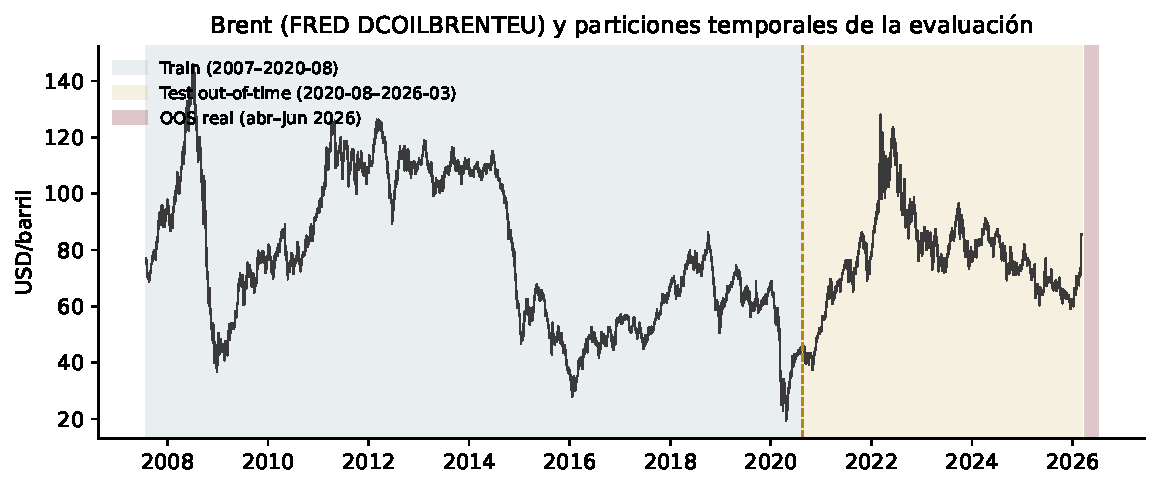
\includegraphics[width=0.98\textwidth]{brent_timeline.pdf}
    \caption{Serie del Brent (FRED) y particiones temporales: entrenamiento hasta
    agosto de 2020, evaluación \emph{out-of-time} 2020--2026 y \emph{test
    out-of-sample} genuino sobre abril--junio de 2026.}
    \label{fig:timeline}
\end{figure}

\subsection{Particiones temporales}
El protocolo usa tres niveles de exigencia creciente:
\begin{itemize}
  \item \textbf{Out-of-time histórico}: corte en 2020-08-20; 4.712 ventanas de
        entrenamiento y 1.974 de test que incluyen el COVID, la guerra de Ucrania
        y los ciclos 2023--2025. Es el escenario base de todas las comparativas.
  \item \textbf{Rolling-origin}: 65 cortes sucesivos para medir la degradación
        del AUC en función de la edad del modelo (Sección~\ref{sec:recalib}).
  \item \textbf{Out-of-sample real}: el detector se entrena solo con datos hasta
        el 6 de marzo de 2026 y se evalúa sobre 83 sesiones de abril--junio de
        2026 descargadas posteriormente de FRED, nunca vistas en ninguna fase de
        diseño (Sección~\ref{sec:oos}).
\end{itemize}

% =============================================================================
\section{Metodología}
% =============================================================================
\subsection{Etiquetado débil geométrico}
\label{sec:etiquetado}
El \emph{bundle} no contiene etiquetas de patrón; estas se generan con reglas
geométricas sobre la trayectoria del Brent dentro de cada ventana de 32 días
(suavizado por media móvil de 3 puntos, detección de extremos locales y
puntuaciones por figura). Las ocho clases candidatas son \texttt{double\_bottom},
\texttt{double\_top}, \texttt{ascending\_channel}, \texttt{descending\_channel},
\texttt{high\_tight\_flag}, \texttt{head\_shoulders},
\texttt{inverse\_head\_shoulders} y \texttt{range}. Una ventana recibe la clase
de máxima puntuación si su confianza supera el umbral (0.35 en el \emph{pipeline}
base; 0.30 en el detector binario); en caso contrario queda sin clasificar. Para
el canal ascendente, por ejemplo, la puntuación combina el signo de la pendiente
del ajuste lineal, su $R^2$, la compacidad de los residuos y la presencia de
oscilaciones internas (formulación completa en el Anexo~\ref{ap:etiquetado}).

Este esquema es una forma de \emph{supervisión débil} \cite{lo2000foundations}:
las etiquetas son un \emph{proxy} reglado y reproducible de lo que un analista
técnico marcaría, no una verdad externa. Las métricas deben leerse, por tanto,
como concordancia del modelo visual con el etiquetador geométrico, evaluada
siempre fuera de la muestra de entrenamiento.

\begin{figure}[H]
    \centering
    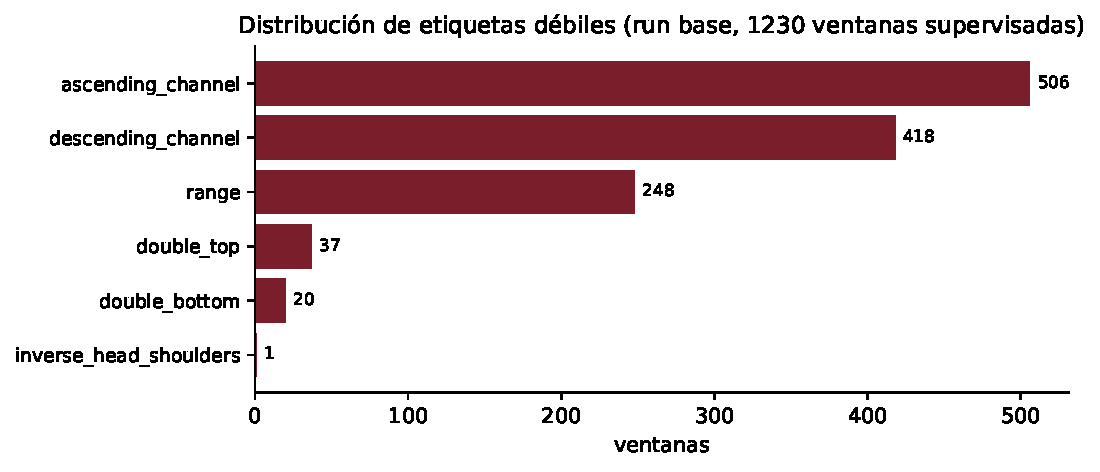
\includegraphics[width=0.78\textwidth]{weak_label_distribution.pdf}
    \caption{Distribución de etiquetas débiles en el run base reproducible. El
    desbalance es estructural: los canales y el rango dominan; las figuras de
    vuelta son marginales en el Brent.}
    \label{fig:labels}
\end{figure}

\subsection{Codificación de la ventana como imagen}
Cada ventana se transforma en una imagen RGB de $160\times160$: canal rojo, GASF
del nivel del Brent; canal verde, GADF de los retornos; canal azul, mapa
multivariante de las variables estandarizadas (o, en la variante solo-precio, de
la propia serie del Brent). La formulación exacta —reescalados, transformación
angular, normalización e interpolación bilineal— se recoge en el
Anexo~\ref{ap:encoding}.

\begin{figure}[H]
    \centering
    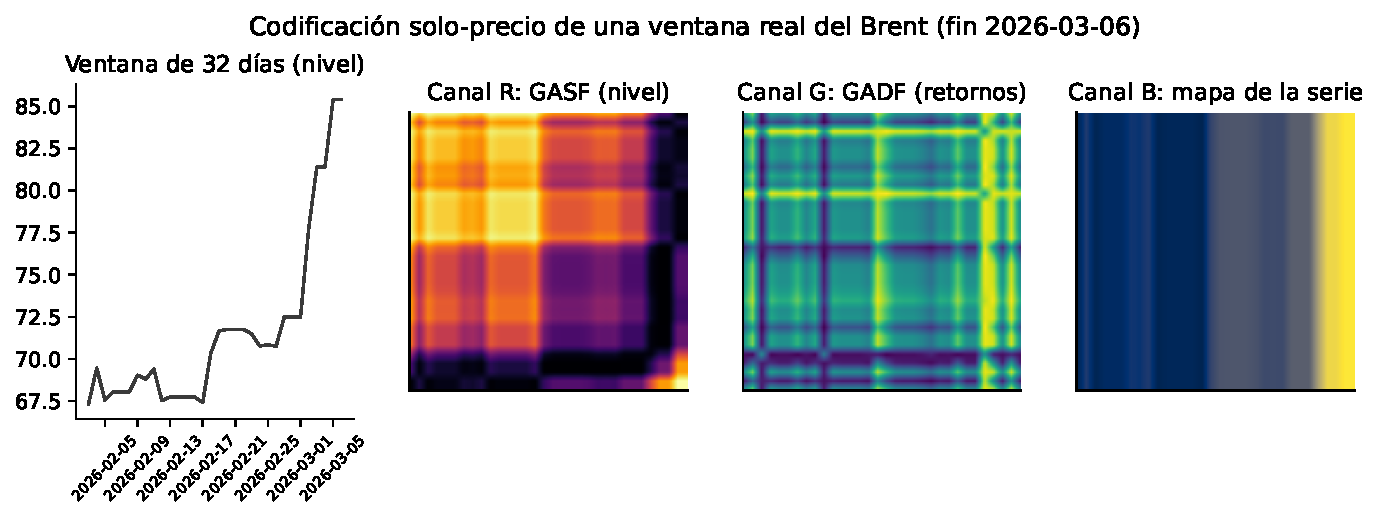
\includegraphics[width=0.98\textwidth]{rgb_channels_example.pdf}
    \caption{Codificación solo-precio de una ventana real del Brent (fin
    2026-03-06): nivel de la serie y los tres canales GASF/GADF/mapa.}
    \label{fig:rgb}
\end{figure}

\subsection{Arquitecturas evaluadas}
\label{sec:arquitecturas}
\paragraph{CNN multitarea (v2).} EfficientNet-B1 con cabeza compartida de 256
unidades (SiLU + \emph{dropout}) y dos ramas: clasificación de 8 patrones y
regresión de tres magnitudes (\texttt{future\_return}, \texttt{future\_low},
\texttt{future\_high}). Pérdida $\mathcal{L}=\mathcal{L}_{\mathrm{cls}} +
\lambda\,\mathcal{L}_{\mathrm{reg}}$ con $\lambda=0.5$, pesos de clase
balanceados o \emph{focal loss} \cite{lin2017focal}, entrenamiento en dos fases
(cabeza con \emph{backbone} congelado; \emph{fine-tuning} de los últimos bloques)
y preentrenamiento sintético opcional de la cabeza con plantillas de patrón.

\paragraph{Detector de canal (v3).} El resultado central del proyecto usa una
arquitectura deliberadamente más simple: EfficientNet-B1 \emph{congelado} (pesos
ImageNet) como extractor de características de la imagen solo-precio, seguido de
una \textbf{regresión logística por patrón} (uno-contra-resto para canal
ascendente y descendente) con pesos de clase balanceados. Esta separación
(representación fija + cabeza lineal) reduce drásticamente el riesgo de
sobreajuste con $\sim$4.700 ventanas de entrenamiento, hace la recalibración
casi instantánea y facilita la trazabilidad del modelo ante terceros. El
artefacto entregado (\texttt{results/models/detector\_canal\_heads.joblib}) es
reproducible con \texttt{code/channel\_detector.py}.

\begin{figure}[H]
    \centering
    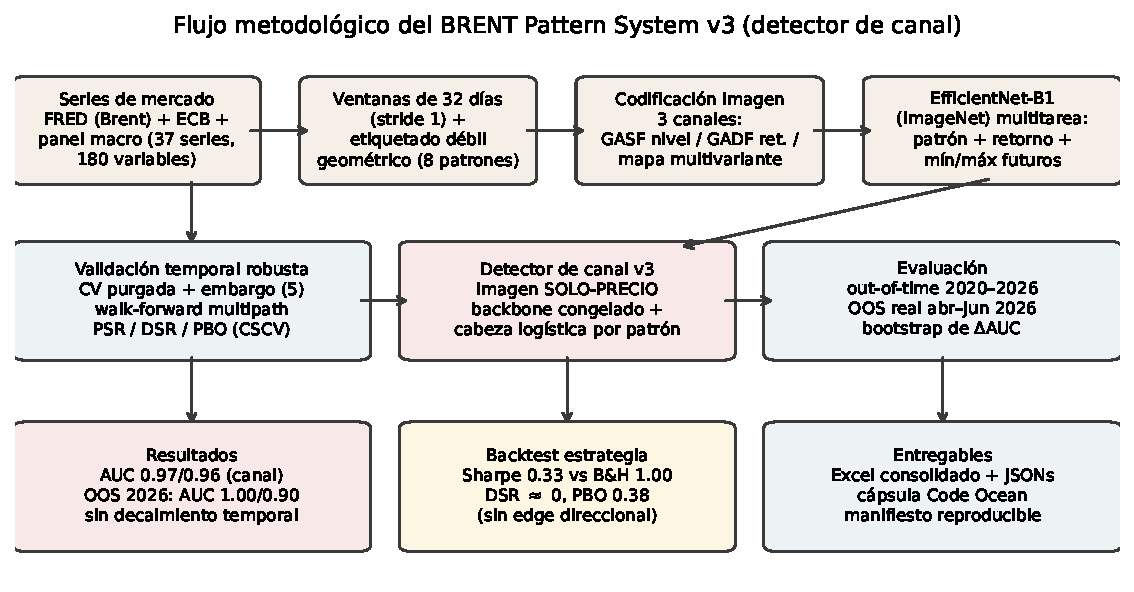
\includegraphics[width=0.98\textwidth]{pipeline_diagram.pdf}
    \caption{Flujo metodológico completo del sistema.}
    \label{fig:pipeline}
\end{figure}

\subsection{Protocolo de validación temporal}
\label{sec:validacion}
Las ventanas se generan con \emph{stride} 1, de modo que dos ventanas contiguas
comparten 31 de 32 observaciones y cada etiqueta depende además de hasta 5 días
futuros. Sin correcciones, cualquier partición aleatoria —e incluso un simple
\emph{holdout} contiguo— filtra información entre entrenamiento y test. El
proyecto aplica el marco de López de Prado \cite{lopezdeprado2018advances}:

\begin{itemize}
  \item \textbf{Purga}: se elimina del entrenamiento toda ventana cuyo intervalo
        de información $[\mathrm{start}_i,\ \mathrm{end}_i - 1 + h_{\max}]$ se
        solape con el de cualquier ventana de validación o test.
  \item \textbf{Embargo}: se descartan además las ventanas dentro de las 5
        posiciones posteriores (e inmediatamente anteriores) a cada bloque de
        evaluación, contra la correlación serial residual.
  \item \textbf{Walk-forward multipath}: el eje temporal se divide en bloques de
        test consecutivos; para cada uno se entrena con el pasado purgado y las
        predicciones \emph{out-of-sample} se concatenan en una única trayectoria.
  \item \textbf{Corrección por sesgo de selección}: sobre la trayectoria agregada
        se calculan PSR, DSR y PBO/CSCV \cite{bailey2012sharpe,bailey2014deflated,
        bailey2017probability} (formulación en el Anexo~\ref{ap:metricas-fin}).
\end{itemize}

% =============================================================================
\section{Resultados}
% =============================================================================
\subsection{Run base reproducible: la línea de base honesta}
\label{sec:runbase}
La cápsula de código reproduce en CPU un \emph{walk-forward} purgado de 3
\emph{folds} de la CNN multitarea sobre el histórico corto (2019--2026, 180
variables, régimen de entrenamiento reducido). El resultado es deliberadamente
modesto —exactitud 0.357, \emph{balanced accuracy} 0.201, macro-F1 0.181 sobre
922 ventanas OOS; DSR 0.084 y PBO 0.729 en el \emph{backtest} direccional— y
cumple dos funciones: valida funcionalmente el \emph{pipeline} de extremo a
extremo en un entorno determinista y deja constancia de que, sin histórico
extendido ni ajustes, el problema multiclase con 8 patrones es difícil. Todos los
experimentos siguientes se construyen sobre esta base con el histórico de la
Sección~\ref{sec:historia}.

\subsection{Detector de canal \emph{out-of-time}: el contexto multiactivo sobra}
\label{sec:crossasset}
La Tabla~\ref{tab:comparativa} y la Figura~\ref{fig:comparativa} comparan cuatro
variantes del detector binario sobre el mismo test \emph{out-of-time}
(2020-08 $\to$ 2026-03, $n=1.974$): la imagen 3-canal completa (con el mapa
multivariante de 180 variables), la imagen solo-precio, una arquitectura de dos
ramas (imagen + vector tabular con 34 correlaciones y retornos
\emph{cross-asset}: DAX, S\&P~500, EURUSD, oro, VIX, tipos, \dots) y la rama
tabular sola.

\begin{table}[H]
\centering
\footnotesize
\caption{Comparativa de variantes del detector de canal (out-of-time, test
2020--2026, $n=1.974$).}
\label{tab:comparativa}
\begin{tabular}{llrrrr}
\toprule
\textbf{Variante} & \textbf{Patrón} & \textbf{AUC} & \textbf{F1} & \textbf{Prec.} & \textbf{Recall} \\
\midrule
Solo-precio (\textbf{mejor}) & ascendente  & \textbf{0.973} & \textbf{0.900} & 0.876 & 0.925 \\
Imagen 3-canal (macro)       & ascendente  & 0.947 & 0.848 & 0.791 & 0.914 \\
Imagen + tabular             & ascendente  & 0.934 & 0.835 & 0.800 & 0.873 \\
Tabular \emph{cross-asset} sola & ascendente & 0.504 & 0.556 & 0.400 & 0.913 \\
\midrule
Solo-precio (\textbf{mejor}) & descendente & \textbf{0.956} & \textbf{0.844} & 0.867 & 0.822 \\
Imagen 3-canal (macro)       & descendente & 0.929 & 0.803 & 0.835 & 0.774 \\
Imagen + tabular             & descendente & 0.909 & 0.776 & 0.784 & 0.769 \\
Tabular \emph{cross-asset} sola & descendente & 0.468 & 0.398 & 0.321 & 0.524 \\
\bottomrule
\end{tabular}
\end{table}

\begin{figure}[H]
    \centering
    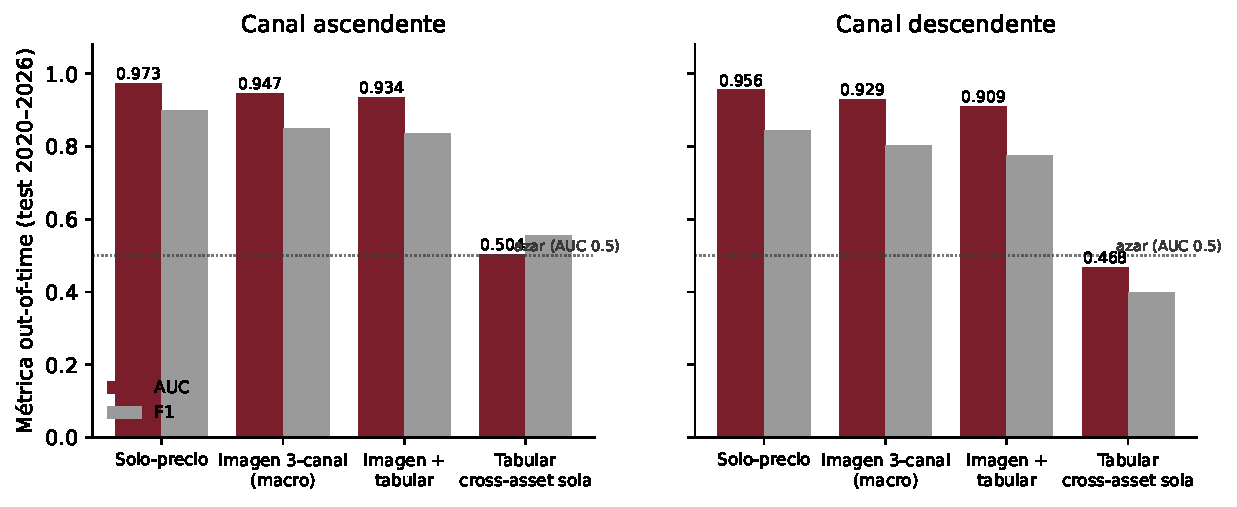
\includegraphics[width=0.98\textwidth]{comparativa_variantes.pdf}
    \caption{AUC y F1 por variante y patrón en el test \emph{out-of-time}. La
    rama tabular \emph{cross-asset} sola es indistinguible del azar.}
    \label{fig:comparativa}
\end{figure}

Tres lecturas. Primera: la rama tabular \emph{cross-asset} aislada rinde al nivel
del azar (AUC 0.50/0.47), pese a que la correlación histórica Brent--EURUSD ronda
0.5 —correlación de \emph{retornos} no es información sobre la \emph{geometría}
local del precio—. Segunda: combinar la imagen con la rama tabular \emph{empeora}
a la imagen sola: el canal adicional actúa como ruido que diluye la señal
morfológica. Tercera: eliminar también el mapa macro del tercer canal (variante
solo-precio) produce la mejor detección en ambos patrones.

Para elevar esta observación a afirmación estadística, se estimó la distribución
de $\Delta\mathrm{AUC} = \mathrm{AUC}_{\text{solo-precio}} -
\mathrm{AUC}_{\text{rival}}$ mediante \emph{bootstrap} estratificado con
$B=3000$ remuestreos del conjunto de test (Anexo~\ref{ap:bootstrap}). Todos los
intervalos de confianza al 95\% excluyen el cero (Figura~\ref{fig:bootstrap}) y
la probabilidad empírica de que el modelo solo-precio gane es del 100\%.

\begin{figure}[H]
    \centering
    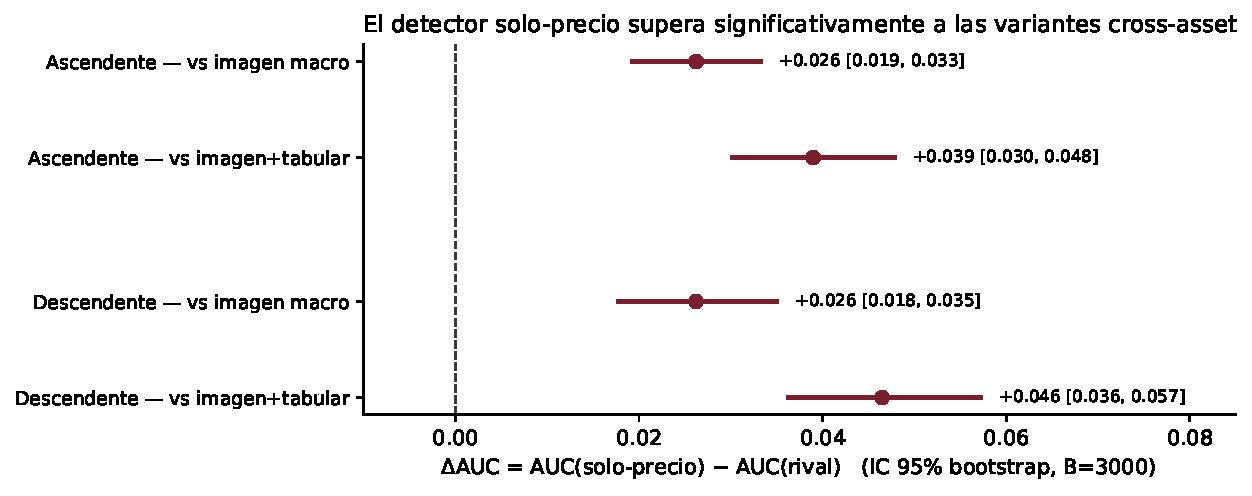
\includegraphics[width=0.9\textwidth]{bootstrap_delta_auc.pdf}
    \caption{Intervalos de confianza \emph{bootstrap} (95\%, $B=3000$) de la
    diferencia de AUC entre el detector solo-precio y cada rival. Frente a la
    rama tabular sola, $\Delta$AUC es $+0.470$ (ascendente) y $+0.488$
    (descendente), fuera de la escala del gráfico.}
    \label{fig:bootstrap}
\end{figure}

\subsection{Test \emph{out-of-sample} real: abril--junio de 2026}
\label{sec:oos}
El detector entrenado con datos hasta 2026-03-06 se aplicó a 83 sesiones
posteriores (2026-04-08 a 2026-06-29) descargadas de FRED tras cerrar el diseño.
Para evitar mezcla de \emph{vintages} (FRED difiere del CSV original en
$\sim$1.19\,USD de media), FRED se usó como fuente única en entrenamiento y test.

\begin{table}[H]
\centering
\footnotesize
\caption{Out-of-sample real abril--junio 2026 ($n=83$; umbral calibrado en
entrenamiento).}
\label{tab:oos}
\begin{tabular}{lrrrrrrr}
\toprule
\textbf{Patrón} & \textbf{Positivos} & \textbf{AUC} & \textbf{Acc.} & \textbf{F1} & \textbf{Prec.} & \textbf{Recall} & \textbf{Umbral} \\
\midrule
Canal ascendente  & 9  & 1.000 & 0.976 & 0.875 & 1.000 & 0.778 & 0.525 \\
Canal descendente & 49 & 0.902 & 0.819 & 0.851 & 0.827 & 0.878 & 0.575 \\
\bottomrule
\end{tabular}
\end{table}

\begin{figure}[H]
    \centering
    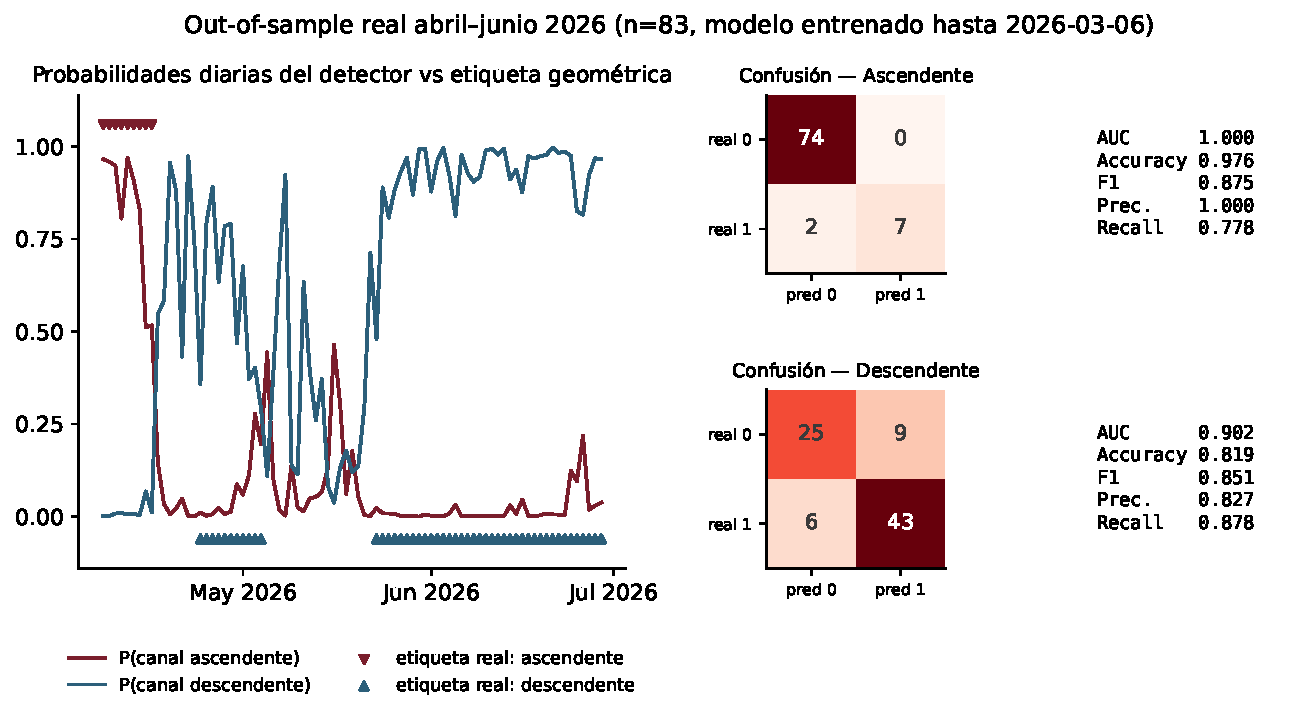
\includegraphics[width=0.98\textwidth]{oos_2026.pdf}
    \caption{OOS real: probabilidades diarias del detector frente a la etiqueta
    geométrica, matrices de confusión y métricas.}
    \label{fig:oos}
\end{figure}

Con la cautela de una muestra de tres meses, el resultado confirma que el modelo
entrenado hasta marzo generaliza al trimestre siguiente sin recalibración: la
detección de canal no es un artefacto del periodo de entrenamiento.

\subsection{Estabilidad temporal y frecuencia de recalibración}
\label{sec:recalib}
Sobre 65 cortes \emph{rolling-origin} se midió el AUC \emph{out-of-sample} en
función de la edad del modelo (tiempo desde el último reentrenamiento). No hay
decaimiento —de hecho el AUC mejora ligeramente con ventanas de evaluación más
largas— lo que indica que la geometría del canal es esencialmente invariante al
régimen de mercado. Operativamente, una recalibración anual de la cabeza
logística es suficiente; la adaptación rápida a \emph{shocks} solo sería
relevante para magnitudes que este sistema no predice (dirección, volatilidad).

\begin{figure}[H]
    \centering
    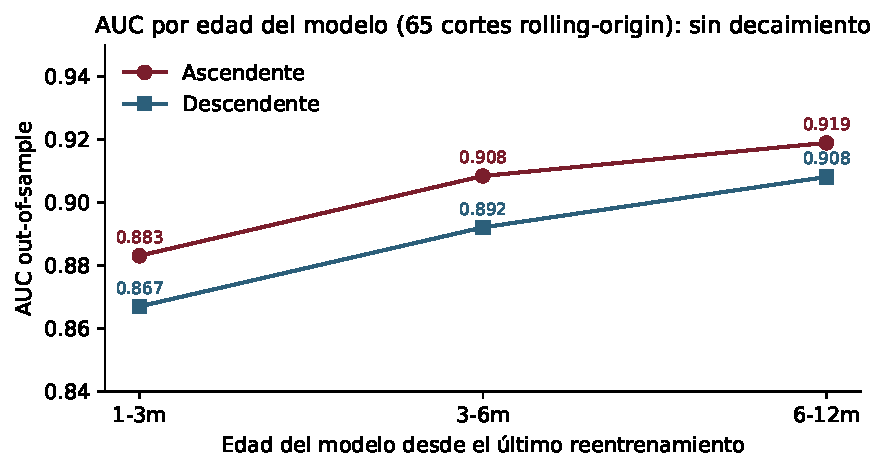
\includegraphics[width=0.7\textwidth]{recalibracion.pdf}
    \caption{AUC por edad del modelo (65 cortes \emph{rolling-origin}): sin
    decaimiento hasta 12 meses.}
    \label{fig:recalib}
\end{figure}

Coherente con lo anterior, una ventana adaptativa por régimen no aporta: la
combinación multi-escala (16/32/64 días) empata con la ventana fija de 32 días y
el \emph{gating} por régimen de volatilidad empeora claramente al fragmentar los
datos (Figura~\ref{fig:adaptativa}).

\begin{figure}[H]
    \centering
    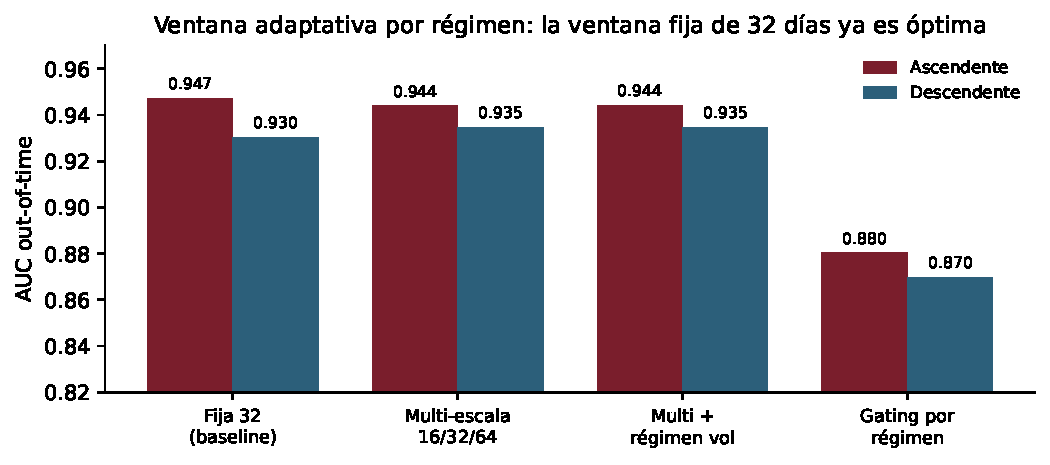
\includegraphics[width=0.9\textwidth]{ventana_adaptativa.pdf}
    \caption{Ventana adaptativa por régimen frente a la ventana fija de 32 días
    (AUC \emph{out-of-time}).}
    \label{fig:adaptativa}
\end{figure}

\subsection{Chartismo por capas: qué patrones son detectables}
\label{sec:multipatron}
Extendiendo el esquema binario a las ocho clases del etiquetador
(Figura~\ref{fig:multipatron}): los canales son detectables con AUC 0.96--0.97;
el rango es detectable con AUC 0.83; el doble techo/suelo emite señal débil
(AUC 0.64--0.68) pero sin utilidad operativa (F1 $=0$ con $\sim$100 casos); y las
figuras hombro-cabeza-hombro y banderas son directamente inexistentes en el Brent
con este etiquetador (soporte 1--6 casos en 6.726 ventanas). El cuello de botella
de la ``capa 2'' del chartismo no es el modelo sino la \emph{frecuencia} real de
esas figuras y la cobertura del etiquetador geométrico.

\begin{figure}[H]
    \centering
    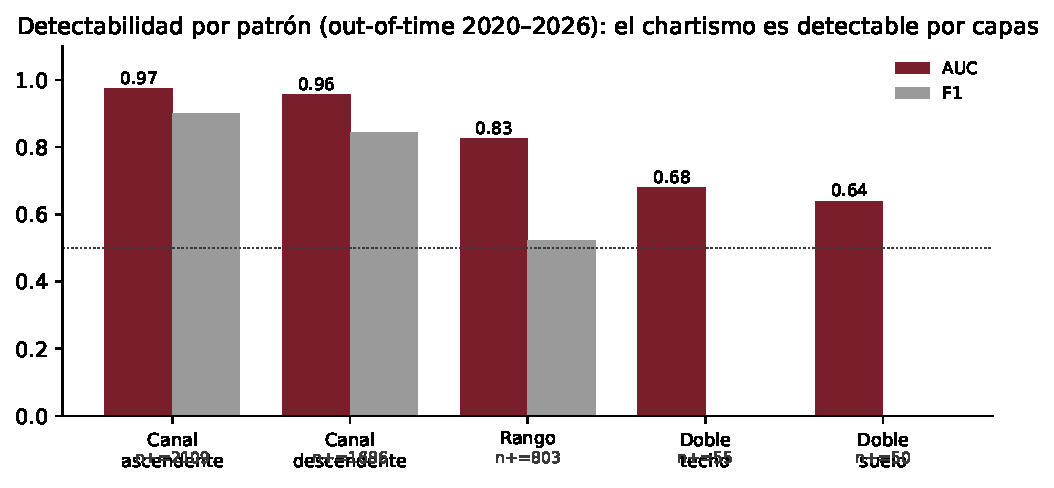
\includegraphics[width=0.92\textwidth]{multipatron.pdf}
    \caption{Detectabilidad por patrón (out-of-time 2020--2026). Bajo cada barra,
    el número de positivos de entrenamiento.}
    \label{fig:multipatron}
\end{figure}

\subsection{Del patrón a la estrategia: el \emph{backtest} que no pasa}
\label{sec:backtest}
¿Se traduce un detector de canal con AUC 0.97 en una estrategia rentable? La
estrategia evaluada toma posición larga en canal ascendente y corta en canal
descendente sobre un tramo OOS \emph{no solapado} de 395 sesiones (2020--2026).
El resultado es negativo de forma robusta (Figura~\ref{fig:backtest}): retorno
acumulado del $+1.7\%$ frente al $+97.1\%$ del \emph{buy \& hold}; Sharpe 0.33
frente a 1.00; y, tras deflactar por las 7 configuraciones probadas
\cite{bailey2014deflated}, un DSR de $1.7\times10^{-6}$ —la probabilidad de que
el Sharpe verdadero supere al máximo esperable por azar es esencialmente nula—.
El PBO (CSCV con 12.870 combinaciones) es 0.38.

\begin{figure}[H]
    \centering
    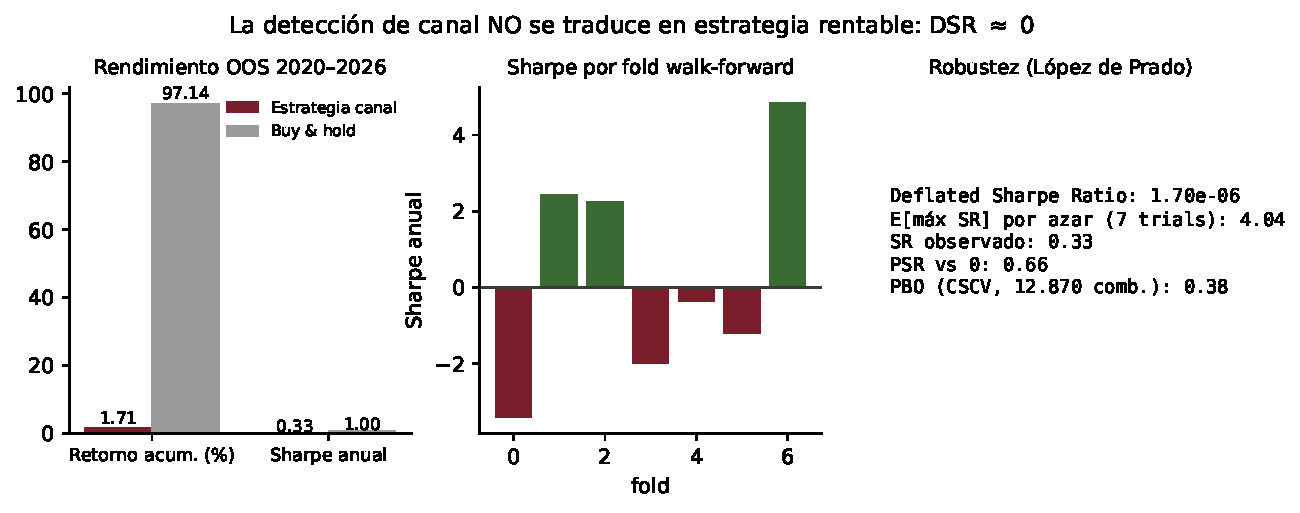
\includegraphics[width=0.98\textwidth]{backtest_canal.pdf}
    \caption{Backtest de la estrategia de canal: rendimiento frente a
    \emph{buy \& hold}, dispersión del Sharpe por \emph{fold} y métricas de
    robustez de López de Prado.}
    \label{fig:backtest}
\end{figure}

Este resultado es coherente con los experimentos direccionales previos: el signo
del retorno \emph{forward} a 5, 10 y 20 días no supera la tasa base en ningún
horizonte (\emph{hit rate} 0.48--0.51 frente a tasas base 0.53--0.55, correlación
$\approx 0$), ni siquiera triplicando el histórico de entrenamiento; y la
volatilidad futura, que sí es predecible, no la captura la CNN (correlación
$\approx 0$) mientras una persistencia trivial alcanza correlaciones de
0.32--0.45. La conclusión metodológica es nítida: \textbf{reconocer la geometría
no equivale a anticipar el movimiento}, exactamente el patrón que cabría esperar
bajo eficiencia débil del mercado \cite{lo2000foundations,white2000reality}.

% =============================================================================
\section{Discusión}
% =============================================================================
\paragraph{Para la función de riesgos.} El sistema entrega una capa de chartismo
objetiva, versionada y auditable: cada señal diaria lleva probabilidades
calibradas por patrón, el artefacto es reproducible desde la cápsula y la
frecuencia de recalibración está justificada empíricamente (anual). El uso
apropiado es descriptivo y de vigilancia —contextualizar el régimen del precio,
alimentar cuadros de mando, priorizar revisión humana— y no la generación de
señales de inversión, extremo que el propio proyecto refuta con DSR $\approx 0$.
Esta separación entre capacidad descriptiva y ausencia de ventaja direccional es
precisamente el tipo de afirmación que los marcos de gobernanza de modelos
(BCBS~239, guía de modelos internos del BCE \cite{bcbs239,ecb2025guide}) exigen
documentar.

\paragraph{Sobre el papel del \emph{cross-asset}.} El resultado más
contraintuitivo es que el contexto multiactivo degrade la detección. La
explicación es informacional: el canal es una propiedad \emph{local y
morfológica} de la serie objetivo; las correlaciones con EURUSD ($\rho \approx
0.5$ histórica), índices o tipos operan a la frecuencia de los retornos y no
restringen la forma de la trayectoria. Añadirlas al tensor de entrada consume
capacidad del modelo en direcciones ortogonales a la tarea. El lugar natural de
la información \emph{cross-asset} serían las tareas direccionales o de riesgo
—que resultaron no predecibles con este esquema— no la geometría.

\paragraph{Limitaciones.} (i) Las etiquetas son débiles: miden concordancia con
un etiquetador geométrico, no con una verdad externa; cambiar sus umbrales
desplaza las métricas. (ii) El OOS real cubre solo un trimestre. (iii) El
etiquetador solo define 8 figuras; triángulos, cuñas, banderines o taza-con-asa
requieren nuevas reglas geométricas. (iv) Las salidas continuas de la CNN
multitarea (\texttt{future\_low}/\texttt{future\_high}) se estiman sin
restricción de orden y ocasionalmente se invierten. (v) El run reproducible en
CPU es un régimen corto: valida el \emph{pipeline}, no el techo de rendimiento.

% =============================================================================
\section{Conclusiones}
% =============================================================================
Un detector de canales sobre el Brent construido con codificación
imagen-de-series (GASF/GADF), un \emph{backbone} EfficientNet-B1 congelado y
cabezas logísticas alcanza AUC de 0.973/0.956 \emph{out-of-time} y generaliza a
un \emph{out-of-sample} genuino de 2026 usando únicamente el precio del activo.
La evidencia \emph{bootstrap} descarta que el contexto \emph{cross-asset} aporte
a esta tarea; la estabilidad temporal permite recalibración anual; y el
\emph{backtest} deflactado demuestra que la detección, siendo casi perfecta, no
constituye ventaja direccional. El valor del proyecto es doble: un componente de
chartismo automatizado listo para integración en procesos de riesgo, y una
demostración metodológicamente rigurosa —CV purgada, DSR, PBO— de los límites
reales del chartismo como fuente de \emph{alpha}.

% =============================================================================
\appendix
% =============================================================================
\section{Formulación matemática del sistema}
\label{ap:matematica}

\subsection{Ventana de entrada y notación}
Sea $\mathbf{b} = (b_1,\dots,b_L) \in \mathbb{R}^{L}$ la serie de precios del
Brent dentro de la ventana $n$-ésima, con $L=32$, y sea
$\mathbf{W}^{(n)} \in \mathbb{R}^{L\times F}$ la matriz multivariante de la
ventana cuando se usa el canal macro ($F=180$ variables estandarizadas). El
objetivo continuo asociado es el log-retorno \emph{forward} a un día
$y^{(n)} = \log(b^{(n)}_{L+1}/b^{(n)}_{L})$, junto con el mínimo y máximo
relativos del corredor futuro de $h_{sr}=5$ días.

\subsection{Etiquetado débil geométrico}
\label{ap:etiquetado}
Sobre la serie suavizada $\tilde{\mathbf{b}} = \mathrm{MA}_3(\mathbf{b})$ se
identifican extremos locales $\{M_j\}$ (máximos) y $\{m_j\}$ (mínimos) con
separación mínima de 3 observaciones. Con el ajuste lineal
$\tilde b_t \approx \alpha + \beta t$, el coeficiente de determinación $R^2$, la
desviación de los residuos $\sigma_\varepsilon$ y el rango
$\rho = \max(\tilde{\mathbf{b}})-\min(\tilde{\mathbf{b}})$, la puntuación del
canal ascendente es
\begin{equation}
s_{\mathrm{asc}} = 0.40\,\mathbf{1}[\beta>0]
 + 0.30\,\max(R^2,0)
 + 0.20\Bigl(1-\min\bigl(\tfrac{\sigma_\varepsilon}{\rho},1\bigr)\Bigr)
 + 0.10\,\min\Bigl(\tfrac{|\{M_j\}|+|\{m_j\}|}{8},1\Bigr),
\end{equation}
y $s_{\mathrm{desc}}(\mathbf{b}) = s_{\mathrm{asc}}(-\mathbf{b})$. Las restantes
figuras (dobles techos/suelos, hombro-cabeza-hombro, bandera, rango) usan
combinaciones análogas de similitud entre extremos, retrocesos y confirmación
final. La etiqueta es $\ell = \arg\max_k s_k$ si
$s_{\ell} \geq \tau$ (con $\tau=0.35$ en el \emph{pipeline} base y $\tau=0.30$
en el detector), y ``sin clasificar'' en caso contrario.

\subsection{Codificación GASF/GADF y mapa multivariante}
\label{ap:encoding}
El nivel se reescala a $[-1,1]$,
\begin{equation}
\tilde b_t = 2\,\frac{b_t - \min(\mathbf{b})}{\max(\mathbf{b}) - \min(\mathbf{b})} - 1,
\qquad \phi_t = \arccos(\tilde b_t)\in[0,\pi],
\end{equation}
y los campos angulares de Gram se definen como \cite{wang2015imaging}
\begin{equation}
\mathrm{GASF}_{ij} = \cos(\phi_i + \phi_j), \qquad
\mathrm{GADF}_{ij} = \sin(\psi_i - \psi_j),
\end{equation}
donde $\psi$ es la representación angular del retorno discreto
$r_t = (b_t - b_{t-1})/\max(b_t,\varepsilon)$, $r_1=0$, reescalado a $[-1,1]$.
Cada mapa se normaliza a $[0,1]$ mediante
$\mathcal{N}(A) = (A - \min A)/(\max A - \min A)$ y se redimensiona a
$160\times160$ con un operador de interpolación bilineal separable
$\mathcal{R}_{160}(\cdot)$ implementado como producto de matrices de
interpolación:
\begin{equation}
\mathbf{C}^{(R)} = \mathcal{R}_{160}(\mathcal{N}(\mathrm{GASF})), \qquad
\mathbf{C}^{(G)} = \mathcal{R}_{160}(\mathcal{N}(\mathrm{GADF})).
\end{equation}

Para el tercer canal, cada fila $\mathbf{m}_f$ de
$\mathbf{M}=\mathbf{W}^{\top}$ (trayectoria de la variable $f$) se escala de
forma robusta,
\begin{equation}
\widehat M_{f,t} = \frac{M_{f,t} - \operatorname{mediana}(\mathbf{m}_f)}
{\operatorname{IQR}(\mathbf{m}_f)},
\qquad
\overline M_{f,t} = \operatorname{clip}\!\Bigl(\frac{\widehat M_{f,t}+3}{6},0,1\Bigr),
\qquad
\mathbf{C}^{(B)} = \mathcal{R}_{160}(\overline{\mathbf{M}}).
\end{equation}
En la variante \textbf{solo-precio}, $\mathbf{M}$ se reduce a la propia serie del
Brent ($F=1$). La imagen final es
$\mathbf{I} = 255\cdot\operatorname{stack}(\mathbf{C}^{(R)},\mathbf{C}^{(G)},
\mathbf{C}^{(B)})$, normalizada con las estadísticas de ImageNet antes del
\emph{backbone}:
\begin{equation}
X_{cij} = \frac{I_{cij}/255 - \mu_c}{\sigma_c},
\qquad
\boldsymbol{\mu}=(0.485,0.456,0.406),\quad
\boldsymbol{\sigma}=(0.229,0.224,0.225).
\end{equation}

\subsection{Backbone convolucional y cabezas}
La operación convolucional genérica de la capa $\ell$ es
\begin{equation}
Y^{(\ell)}_{c_o,i,j} = b^{(\ell)}_{c_o} +
\sum_{c_i=1}^{C_{\mathrm{in}}}\sum_{u=0}^{k_h-1}\sum_{v=0}^{k_w-1}
W^{(\ell)}_{c_o,c_i,u,v}\,X^{(\ell-1)}_{c_i,\,i+u,\,j+v},
\qquad
\mathbf{A}^{(\ell)} = \operatorname{SiLU}\bigl(\operatorname{BN}(\mathbf{Y}^{(\ell)})\bigr),
\end{equation}
con $\operatorname{SiLU}(x)=x\,\sigma(x)$. Tras el \emph{global average pooling}
final, $h_c = \frac{1}{HW}\sum_{i,j} A^{(L_b)}_{cij}$, el vector latente es
$\mathbf{h}=f_{\mathrm{EffB1}}(\mathbf{X})\in\mathbb{R}^{1280}$
\cite{tan2019efficientnet}.

\paragraph{CNN multitarea (v2).} Cabeza compartida
$\mathbf{s}=\operatorname{Dropout}(\operatorname{SiLU}(\mathbf{W}_h
\operatorname{Dropout}(\mathbf{h})+\mathbf{b}_h))\in\mathbb{R}^{256}$; logits de
clasificación $\mathbf{z}=\mathbf{W}_c\mathbf{s}+\mathbf{b}_c\in\mathbb{R}^{8}$
con $p_k = e^{z_k}/\sum_j e^{z_j}$; regresión
$\widehat{\mathbf{y}}^{\mathrm{reg}} = \mathbf{W}_r\mathbf{s}+\mathbf{b}_r \in
\mathbb{R}^3$. La pérdida es
\begin{equation}
\mathcal{L} = \mathcal{L}_{\mathrm{cls}} + \lambda\,\mathcal{L}_{\mathrm{reg}},
\qquad \lambda = 0.5,
\end{equation}
con $\mathcal{L}_{\mathrm{cls}}$ la entropía cruzada ponderada por clase
($w_c = N/(K\,n_c)$, normalizados a media 1) o la \emph{focal loss}
\cite{lin2017focal}
\begin{equation}
\mathcal{L}_{\mathrm{focal}} = (1-p_t)^{\gamma}\,\bigl(-\log p_t\bigr),
\qquad \gamma = 2,
\end{equation}
y $\mathcal{L}_{\mathrm{reg}}$ la pérdida SmoothL1 (Huber) media sobre las tres
salidas:
\begin{equation}
\operatorname{SmoothL1}(u)=
\begin{cases}
\tfrac{1}{2}u^2, & |u|<1,\\
|u|-\tfrac{1}{2}, & |u|\ge 1.
\end{cases}
\end{equation}

\paragraph{Detector de canal (v3).} Con el \emph{backbone} congelado, para cada
patrón $k\in\{\text{asc},\text{desc}\}$ se ajusta una regresión logística
binaria
\begin{equation}
\Pr(y_k=1\mid\mathbf{h}) = \sigma(\mathbf{w}_k^{\top}\mathbf{h} + b_k),
\qquad
\min_{\mathbf{w}_k,b_k}\ \sum_{n} \omega_{y_n}\,
\log\bigl(1+e^{-\tilde y_n(\mathbf{w}_k^{\top}\mathbf{h}_n+b_k)}\bigr),
\end{equation}
con $\tilde y_n \in \{-1,+1\}$ y pesos de clase balanceados
$\omega_{y}\propto N/(2\,n_{y})$. La decisión binaria usa el umbral que maximiza
el F1 en entrenamiento (0.525/0.575 en el modelo final).

\subsection{Purga, embargo y walk-forward}
Cada ventana $i$ tiene un intervalo de información
$[\mathrm{left}_i,\ \mathrm{right}_i] = [\mathrm{start}_i,\ \mathrm{end}_i - 1 +
h_{\max}]$ con $h_{\max}=\max(h,\,h_{sr})=5$. El conjunto de entrenamiento purgado
respecto a un bloque de test $T$ es
\begin{equation}
\mathrm{train}^{*} = \{\, i \in \mathrm{train} :
[\mathrm{left}_i,\mathrm{right}_i] \cap
[\min_{j\in T}\mathrm{left}_j,\ \max_{j\in T}\mathrm{right}_j] = \emptyset \,\},
\end{equation}
y el embargo elimina además $\{i : \max(T) < i \leq \max(T)+E\}$ con $E=5$
\cite{lopezdeprado2018advances}. En el \emph{walk-forward}, el eje temporal se
divide en $K{+}1$ bloques; el bloque $b$ ($b\geq 2$) actúa como test con
entrenamiento en el pasado purgado y validación en la cola contigua, y las
predicciones OOS se concatenan en una trayectoria única.

% =============================================================================
\section{Justificación de las métricas de evaluación}
\label{ap:metricas}
Esta sección motiva cada métrica utilizada, anticipando la pregunta natural de
un comité de publicación: \emph{¿por qué estas métricas y no otras?} El criterio
rector es doble: (i) el problema es de \textbf{clasificación con desbalance
fuerte y umbral operativo no fijado a priori}, y (ii) toda afirmación económica
debe corregirse por \textbf{sesgo de selección y solapamiento temporal}.

\subsection{AUC-ROC como métrica primaria de detección}
El AUC (área bajo la curva ROC) admite una interpretación probabilística exacta:
es la probabilidad de que un positivo aleatorio reciba mayor puntuación que un
negativo aleatorio, $\mathrm{AUC} = \Pr(s^{+} > s^{-})$, equivalente al
estadístico de Mann--Whitney \cite{hanley1982meaning}. Tres propiedades lo hacen
idóneo aquí: es \textbf{independiente del umbral de decisión} —crucial porque el
umbral operativo del detector lo fija el usuario de riesgo, no el modelo—; es
\textbf{insensible a la prevalencia}, lo que permite comparar el canal
ascendente (tasa base 0.40) con el descendente (0.33) y con el OOS de 2026 (tasa
0.11) en una escala común; y está estandarizado en la literatura de evaluación de
clasificadores \cite{bradley1997use,fawcett2006introduction}, con el azar
anclado en 0.5. La comparación formal entre AUCs correlacionados (mismo test)
se realiza aquí por \emph{bootstrap} (Sección~\ref{ap:bootstrap}), la
alternativa no paramétrica al test de DeLong \cite{delong1988comparing}.

\subsection{Precisión, recall y F1 en el punto operativo}
El AUC resume el \emph{ranking}; la operación exige un punto concreto. En un
problema desbalanceado, la exactitud es engañosa (predecir ``no canal'' siempre
daría $\sim$60--90\% de acierto), por lo que se reporta la tripleta
precisión--\emph{recall}--F1 \cite{powers2011evaluation,saito2015precision}:
\begin{equation}
\mathrm{Prec} = \frac{TP}{TP+FP}, \qquad
\mathrm{Rec} = \frac{TP}{TP+FN}, \qquad
F1 = \frac{2\,\mathrm{Prec}\cdot\mathrm{Rec}}{\mathrm{Prec}+\mathrm{Rec}}.
\end{equation}
La precisión responde a la pregunta del usuario (``cuando el sistema marca canal,
¿cuánto me puedo fiar?''), el \emph{recall} a la del supervisor (``¿cuántos
canales reales se escapan?'') y el F1 —media armónica— penaliza los desequilibrios
entre ambas, lo que lo convierte en la métrica de selección de umbral. Saito y
Rehmsmeier \cite{saito2015precision} muestran que, con clases desbalanceadas, el
espacio precisión-\emph{recall} es más informativo que el ROC; por ello ambas
familias se reportan conjuntamente.

\subsection{Balanced accuracy y macro-F1 en el problema multiclase}
En la clasificación de 8 patrones, la exactitud global queda dominada por las
clases mayoritarias. La \emph{balanced accuracy} (media de los \emph{recalls} por
clase) corrige exactamente ese sesgo y tiene distribución posterior conocida
\cite{brodersen2010balanced}; el macro-F1 (media no ponderada de los F1 por
clase) obliga al modelo a rendir en las clases raras. Por ese motivo el
\emph{pipeline} selecciona el modelo por macro-F1 en validación
(\texttt{monitor\_metric}) y reporta ambas junto a la matriz de confusión
completa y el soporte por clase —los tres ingredientes que permiten a un revisor
recalcular cualquier métrica derivada—.

\subsection{Intervalos bootstrap para comparar modelos}
\label{ap:bootstrap}
Las diferencias de AUC entre variantes se evalúan con \emph{bootstrap}
estratificado \cite{efron1994introduction}: se remuestrea el conjunto de test
con reemplazo ($B=3000$, preservando la proporción de positivos), se recalcula
$\Delta\mathrm{AUC}^{(b)}$ en cada réplica y se reporta el intervalo percentil
al 95\% junto con $\Pr(\Delta>0)$. Al remuestrear \emph{el mismo} conjunto de
test para ambos modelos se respeta la correlación entre sus errores
—la misma lógica que el test de DeLong \cite{delong1988comparing}— sin asumir
normalidad. Un IC 95\% que excluye el cero equivale a rechazar la igualdad de
AUCs al nivel del 5\%.

\subsection{Métricas económicas corregidas por sesgo de selección}
\label{ap:metricas-fin}
Un Sharpe atractivo puede fabricarse probando configuraciones hasta que una
funcione \cite{white2000reality,harvey2015backtesting}. Por ello el
\emph{backtest} no reporta el Sharpe \cite{sharpe1994ratio} aislado, sino:

\paragraph{PSR.} El \emph{Probabilistic Sharpe Ratio} \cite{bailey2012sharpe}
estima la probabilidad de que el Sharpe verdadero supere un umbral $SR^{*}$,
corrigiendo por longitud de muestra, asimetría $\hat\gamma_3$ y curtosis
$\hat\gamma_4$ de los retornos:
\begin{equation}
\widehat{\mathrm{PSR}}(SR^{*}) =
\Phi\!\left(\frac{(\widehat{SR}-SR^{*})\sqrt{n-1}}
{\sqrt{1-\hat\gamma_3\widehat{SR}+\frac{\hat\gamma_4-1}{4}\widehat{SR}^2}}\right).
\end{equation}

\paragraph{DSR.} El \emph{Deflated Sharpe Ratio} \cite{bailey2014deflated} es el
PSR evaluado contra el máximo Sharpe esperable por puro azar tras $N$ pruebas
con varianza $V$ entre ellas:
\begin{equation}
SR^{*}_{\mathrm{defl}} = \sqrt{V}\left[(1-\gamma_E)\,\Phi^{-1}\!\Bigl(1-\tfrac{1}{N}\Bigr)
 + \gamma_E\,\Phi^{-1}\!\Bigl(1-\tfrac{1}{Ne}\Bigr)\right],
\end{equation}
con $\gamma_E$ la constante de Euler--Mascheroni. En este proyecto $N$ incluye
los \emph{folds} del \emph{walk-forward} y las variantes de señal probadas; el
DSR $\approx 0$ del \emph{backtest} de canal significa que el Sharpe observado
(0.33) es plenamente atribuible a la búsqueda.

\paragraph{PBO.} La \emph{Probability of Backtest Overfitting}
\cite{bailey2017probability} se estima por CSCV: la matriz $T\times N$ de
rendimientos por periodo y configuración se parte en $S=16$ bloques; para cada
una de las $\binom{S}{S/2}=12.870$ combinaciones se elige la mejor configuración
\emph{in-sample} y se observa su rango \emph{out-of-sample}. El PBO es la
frecuencia con que esa mejor configuración cae por debajo de la mediana OOS
(logit $\leq 0$).

\paragraph{Por qué CV purgada y no K-fold.} Con \emph{stride} 1, dos ventanas
adyacentes comparten el 97\% de la información y las etiquetas dependen de hasta
5 días futuros; una CV aleatoria colocaría en entrenamiento réplicas casi exactas
del test, inflando todas las métricas. La purga elimina el solapamiento de
intervalos de información y el embargo la filtración serial residual
\cite{lopezdeprado2018advances}; es la única configuración bajo la cual las
métricas de las secciones \ref{sec:crossasset}--\ref{sec:backtest} son
interpretables como generalización.

\subsection{Resumen de correspondencia métrica--pregunta}
\begin{table}[H]
\centering
\footnotesize
\caption{Cada métrica responde a una pregunta distinta del comité.}
\begin{tabularx}{\textwidth}{lXl}
\toprule
\textbf{Métrica} & \textbf{Pregunta que responde} & \textbf{Referencia} \\
\midrule
AUC-ROC & ¿Ordena bien el detector, sin fijar umbral y sin efecto de la prevalencia? & \cite{hanley1982meaning,fawcett2006introduction} \\
Prec./Recall/F1 & ¿Qué fiabilidad y cobertura tiene el punto operativo elegido? & \cite{saito2015precision,powers2011evaluation} \\
Balanced acc., macro-F1 & ¿Rinde el multiclase también en las clases raras? & \cite{brodersen2010balanced} \\
Bootstrap $\Delta$AUC & ¿Es la mejora entre modelos estadísticamente real? & \cite{efron1994introduction,delong1988comparing} \\
Sharpe + PSR & ¿Es el rendimiento distinguible de cero con no-normalidad? & \cite{sharpe1994ratio,bailey2012sharpe} \\
DSR & ¿Sobrevive el rendimiento a la corrección por número de pruebas? & \cite{bailey2014deflated,harvey2015backtesting} \\
PBO (CSCV) & ¿Con qué probabilidad la mejor config. IS falla OOS? & \cite{bailey2017probability} \\
CV purgada + embargo & ¿Están las métricas libres de fuga por solapamiento? & \cite{lopezdeprado2018advances} \\
\bottomrule
\end{tabularx}
\end{table}

% =============================================================================
\section{Reproducibilidad}
\label{ap:repro}
% =============================================================================
El sistema se distribuye como cápsula tipo Code Ocean
(\texttt{code/}, \texttt{data/}, \texttt{environment/}, \texttt{metadata/},
\texttt{results/}) con entorno fijado por \texttt{Dockerfile} y
\texttt{requirements.txt}, semillas deterministas (\texttt{seed}=42,
\texttt{PYTHONHASHSEED}=0) y ejecución offline en CPU
(\texttt{pretrained\_backbone}=false en el run base). La configuración del
experimento vive en ficheros externos (\texttt{config\_codeocean.\{json,yaml\}},
\texttt{config\_gpu.yaml}); cada run emite un manifiesto
(\texttt{results/reports/run\_manifest.json}) con la configuración resuelta, las
versiones del entorno y el \emph{commit} de git, además de un libro Excel con
todas las métricas y parámetros para validación por revisores.

El detector de canal se reproduce con:
\begin{verbatim}
python code/channel_detector.py train --config code/config_codeocean.yaml \
       --cutoff 2020-08-20      # reproduce detector_solo_precio.json
python code/channel_detector.py predict --prices brent.csv --out preds.csv
\end{verbatim}
Los resultados citados en este documento corresponden a los ficheros de
\texttt{results/reports/} (\texttt{detector\_solo\_precio.json},
\texttt{argumento\_precio\_vs\_crossasset.json},
\texttt{oos\_reciente\_2026.json}, \texttt{detector\_canal\_out\_of\_time.json},
\texttt{dos\_ramas\_crossasset.json}, \texttt{multipatron.json},
\texttt{ventana\_adaptativa.json}, \texttt{backtest\_canal\_dsr\_pbo.json}) y al
Excel consolidado \texttt{brent\_canal\_resultados.xlsx}.

\bibliographystyle{unsrtnat}
\bibliography{references}

\end{document}
